\documentclass[xcolor=svgnames,t]{beamer} 
\usepackage[utf8]{inputenc}
\usepackage{booktabs, comment}
\usepackage{graphicx}  % Add graphicx package
\usepackage[absolute, overlay]{textpos} 
\usepackage{pgfpages}
\usepackage[font=footnotesize]{caption}
\useoutertheme{infolines} 
\usepackage{xcolor}
% \usepackage{cite}  % REMOVE this line because it conflicts with natbib
\usepackage{colortbl}
\definecolor{brownbrown}{RGB}{8, 8, 9}
\usepackage[round, sort, authoryear]{natbib}  % Use only natbib for citation management
\definecolor{brownred}{RGB}{198, 198, 198}

\setbeamercolor{title in head/foot}{bg=brownred, fg=brownbrown}
\setbeamercolor{author in head/foot}{bg=myuniversity}
\setbeamertemplate{page number in head/foot}{}

\usepackage{amsmath}
\usepackage[makeroom]{cancel}

\newtheorem{equi}{} %Creates a grey box when equi is called
\setbeamertemplate{navigation symbols}{} 
\usepackage{textpos}

\usepackage{tikz}

\usetheme{Madrid}
\definecolor{myuniversity}{RGB}{48, 67, 180}
\usecolortheme[named=myuniversity]{structure}
\usepackage{tikz}


\usepackage{colortbl} 
\newcommand{\myitem}{\item[$\circ$]}
\newcommand{\witem}{\item[\textcolor{white}{$\bullet$}]}
\DeclareMathOperator*{\argmax}{arg\,max}
\DeclareMathOperator*{\argmin}{arg\,min}
\AtBeginSection[]{
\begin{frame}
\frametitle{Content}
\tableofcontents[currentsection]
\end{frame}
}

\title[High Dimensionality and DML]{High Dimensionality and Double Machine Learning}
\subtitle{}
%\titlegraphic{\includegraphics[height=1cm]{brown-logo.png}}  % This line is commented out to remove the logo
\author[CIML ]{Causal Inference using Machine Learning\\ Master in Economics, UNT}
\institute[]{Andres Mena}
\date{Spring 2024}

\addtobeamertemplate{navigation symbols}{}{%
    \usebeamerfont{footline}%
    \usebeamercolor[fg]{footline}%
    \hspace{1em}%
    \insertframenumber/\inserttotalframenumber
}

\begin{document}
\begin{frame}
\maketitle
\end{frame}

\section{LASSO Regression and Its Properties}

\begin{frame}{High-Dimensional Linear Regression and LASSO }
\textbf{Setting:} We consider a high-dimensional linear model
\[
Y = \beta'X + \varepsilon, \quad \varepsilon \perp X,
\]
where the dimension of $X$ (denoted $p$) can be very large, possibly much larger than $n$, the sample size.

\pause

\textbf{Challenge:} Ordinary Least Squares (OLS) is prone to overfitting when $p$ is large. High complexity leads to large variance of estimates and poor out-of-sample performance.

\pause

\textbf{Idea of LASSO:} The LASSO estimator imposes a penalty on the size of the coefficients to control complexity:
\[
\widehat{\beta}^{\text{LASSO}} = \arg\min_{b \in \mathbb{R}^p} \sum_{i=1}^n (Y_i - b'X_i)^2 + \lambda \sum_{j=1}^p |b_j|.
\]

\pause

This penalty shrinks some coefficients towards zero, performing both regularization and variable selection.
\end{frame}

\begin{frame}{Bias-Variance Trade-off in LASSO (1)}
    \textbf{Bias-Variance Trade-off:} 
    \begin{itemize}
        \item \textbf{Variance Reduction:} By penalizing large coefficients, LASSO reduces variance in estimates, making predictions more stable.
        \pause
        \item \textbf{Introduction of Bias:} The penalty \(\lambda \sum |b_j|\) shrinks coefficients towards zero. This shrinkage induces bias in the estimates \(\widehat{\beta}^{\text{LASSO}}\) compared to OLS.\\[5pt]
        \[
        |\widehat{\beta}^{\text{LASSO}}| \;\leq\; |\widehat{\beta}^{\text{OLS}}|
        \]
    \end{itemize}
    
    \pause
    
    \begin{center}
    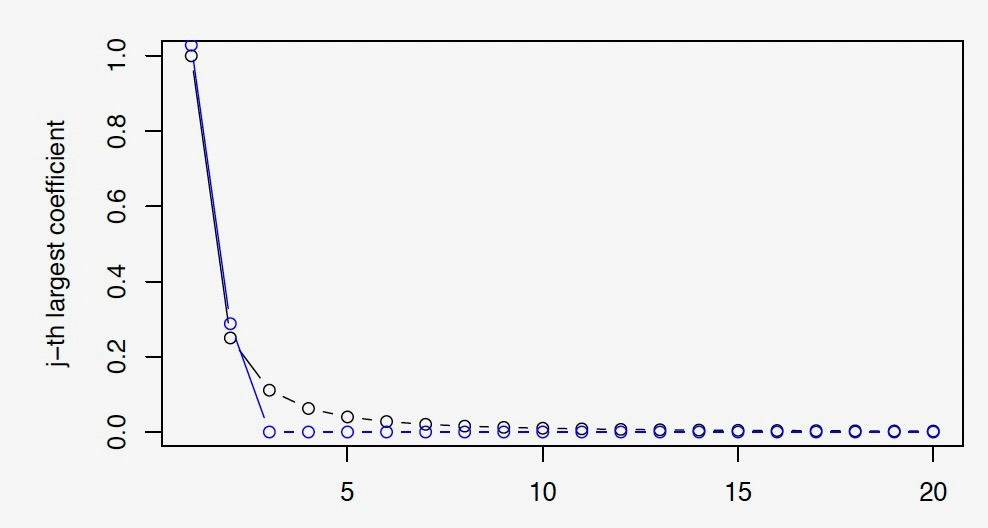
\includegraphics[width=0.6\textwidth]{Figures/bias.jpeg}
    \end{center}
    \end{frame}
    
    
    \begin{frame}{Optimal Penalties: Balancing Bias-Variance and Sparsity}
        \textbf{Optimal Trade-off in LASSO:}
        \begin{itemize}
            \item Carefully choosing \(\lambda\) balances bias and variance.
            \pause
            \item A larger \(\lambda\) increases bias (more shrinkage) but lowers variance.
            \pause
            \item A smaller \(\lambda\) reduces bias but may increase variance.
            \pause
        \end{itemize}
        
        \textbf{Goal:} Find the sweet spot where predictive performance is optimized.
        
        \pause
        
        \textbf{Penalty and Induced Sparsity:}
        \begin{itemize}
            \item LASSO sets coefficients to zero if their marginal predictive benefit does not outweigh the penalty cost.
            \pause
            \item 
            \[
            \widehat{\beta}_j = 0 \text{ if } 
            \left|\frac{\partial}{\partial \widehat{\beta}_j}\sum_{i}(Y_i-\widehat{\beta}'X_i)^2\right| < \lambda.
            \]
            \pause
            \item This condition ensures that only variables with sufficiently high marginal predictive contribution survive the penalty, inducing sparsity in the model.
        \end{itemize}
        \end{frame}
        
    
        \begin{frame}{Predictive Performance of LASSO: Theoretical Guarantees}
            \textbf{Theorem (Predictive Performance of Lasso)}\\[5pt]
            Under approximate sparsity and suitable regularity conditions, if we choose $\lambda$ as recommended (e.g., $\lambda \propto \sigma \sqrt{n\log(\max\{p,n\})}$) and let $s$ be the effective dimension (number of important parameters):
            
            \[
            \sqrt{E_X[(\beta'X - \widehat{\beta}'X)^2]} \leq \text{const} \cdot \sqrt{E[\varepsilon^2]} \sqrt{\frac{s \log(\max\{p,n\})}{n}}.
            \]
            
            Moreover, with high probability:
            \begin{itemize}
                \item The number of regressors selected by LASSO is of order $s$.
                \item If $s \log(\max\{p,n\})/n$ is small, LASSO is close to the best linear predictor.
            \end{itemize}
            
            \pause
            
            \textbf{Implication:} LASSO adapts to unknown sparsity, suffering a modest $\sqrt{\log(\max\{p,n\})}$ factor over the ideal $\sqrt{s/n}$ rate.
            \end{frame}
            
            
            \begin{frame}{Conclusions on LASSO’s Properties}
            \begin{itemize}
                \item \textbf{High Bias in $\widehat{\beta}$:} LASSO deliberately shrinks coefficients, introducing bias relative to OLS.
                \pause
                \item \textbf{Low Variance:} The shrinkage reduces variance, leading to more stable predictions.
                \pause
                \item \textbf{Sparsity:} By setting some coefficients to zero, LASSO performs variable selection and yields parsimonious models.
                \pause
                \item \textbf{Improved Predictive Performance for $Y$:} Despite the bias in $\widehat{\beta}$, the overall prediction $\widehat{\beta}'X$ often outperforms OLS predictions out-of-sample, especially when $p$ is large and $s$ is relatively small.
            \end{itemize}
            
            \textbf{Bottom Line:} LASSO trades off some bias in parameter estimates for substantial gains in predictive stability and interpretability. This is useful for high-dimensional econometric applications.
            \end{frame}
            
            \section{Double LASSO}

            \begin{frame}{Naive Estimator (1)}
                \textbf{Naive Estimator Setup:}
                \begin{itemize}
                    \item Consider two separate LASSO regressions:
                    \[
                    \widehat{\beta}_1 = \arg\min_{\beta_1} \sum_{i:D_i=1}(Y_i - W_i'\beta_1)^2 + \lambda_1 \sum_{j=1}^p |\beta_{1j}|,
                    \]
                    and
                    \[
                    \widehat{\beta}_0 = \arg\min_{\beta_0} \sum_{i:D_i=0}(Y_i - W_i'\beta_0)^2 + \lambda_0 \sum_{j=1}^p |\beta_{0j}|.
                    \]
                
                    \pause
                
                    \item Then form the naive ATE estimator:
                    \[
                    \widehat{\alpha} = \frac{1}{N}\sum_{i=1}^N W_i'(\widehat{\beta}_1 - \widehat{\beta}_0).
                    \]
                \end{itemize}
                \end{frame}
                
                
                \begin{frame}{Naive Estimator (2)}
                \textbf{Neyman Orthogonality and Bias:}
                \begin{itemize}
                    \item The moment condition for the naive estimator is:
                    \[
                    E[W'(\beta_1 - \beta_0) - \alpha] = 0.
                    \]
                
                    \pause
                
                    \item Derivatives w.r.t. $\beta_1$ and $\beta_0$:
                    \[
                    \frac{\partial}{\partial \beta_1}E[W'(\beta_1 - \beta_0) - \alpha] = E[W] \neq 0, \quad
                    \frac{\partial}{\partial \beta_0}E[W'(\beta_1 - \beta_0) - \alpha] = -E[W] \neq 0.
                    \]
                
                    \pause
                
                    \item \textbf{Not Neyman Orthogonal:} Since the derivatives are not zero, the moment condition is not orthogonal. Thus, the estimation error in $(\widehat{\beta}_1 - \widehat{\beta}_0)$ induces slow bias convergence for $\widehat{\alpha}$.
                
                    \pause
                
                    \item \textbf{Consequence:} The bias converges at a slower than $\sqrt{n}$-rate, rendering standard inference methods unreliable for moderate sample sizes.
                \end{itemize}
                \end{frame}
                
                
            
            
            \begin{frame}{Why the Naive Estimator Performs Poorly }
            \begin{center}
            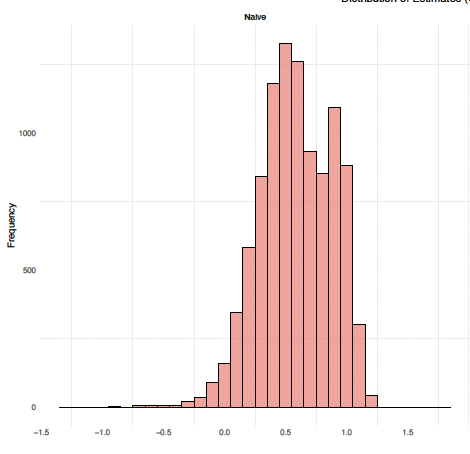
\includegraphics[width=0.45\textwidth]{Figures/naive.png}
            \end{center}
            
            \pause
            \scriptsize
            \textbf{Key Insight:}
            \begin{itemize}
                \item The naive method selects only strong predictors of $Y$.
                \pause
                \item Weak $Y$-predictors that strongly predict $D$ are dropped, causing severe omitted variable bias.
                \pause
                \item The orthogonal approach (Double Lasso) solves two prediction problems (for $Y$ and $D$) and includes controls that matter for either, thus "de-confounding" the residuals.
            \end{itemize}
            
            \pause
            \textbf{Homework:} Replicate CIML Example 4.3.1.
            \end{frame}
            
            
            \begin{frame}{Double Lasso Procedure}
            \textbf{Partialling-Out via Frisch-Waugh-Lovell:}  
            \[
            Y = \alpha D + \beta'W + \epsilon.
            \]
            
            \pause
            
            After partialling out $W$:
            \[
            \tilde{Y} = \alpha \tilde{D} + \tilde{\epsilon}, \quad \text{with } E[\tilde{\epsilon}\tilde{D}] = 0.
            \]
            
            \pause
            
            \textbf{Double Lasso Steps:}
            \begin{enumerate}
                \item Run LASSO: $Y$ on $W$ and $D$ on $W$ to get residuals:
                \[
                    \tilde{Y} = Y - \widehat{\gamma}_{YW}'W,\quad  \tilde{D} = D - \widehat{\gamma}_{DW}'W.
                \]
                \pause
                \item Run OLS of $\tilde{Y}$ on $ \tilde{D}$:
                \[
                \widehat{\alpha} = \frac{\sum  \tilde{D}_i \tilde{Y}_i}{\sum  \tilde{D}_i^2}.
                \]
            \end{enumerate}
            \end{frame}
            
            
            \begin{frame}{Double Lasso Conditions}
            \textbf{Approximate Sparsity:} For good performance, we need the coefficients for $Y$-on-$W$ and $D$-on-$W$ to be approximately sparse:
            \[
            | \gamma_{YW}|_{(j)} \leq A j^{-a}, \quad | \gamma_{DW}|_{(j)} \leq A j^{-a},\quad a>1.
            \]
            
            \pause
            
            \textbf{Tuning:} 
            \begin{itemize}
                \item Choose $\lambda_1, \lambda_2$ (penalties) using theory-driven plug-in rules or related methods.
                \pause
                \item Ensures that the first-step estimation does not have a first-order effect on $\widehat{\alpha}$.
            \end{itemize}
            
            \pause
            
            Without these conditions, and relying solely on cross-validation, performance may suffer in moderate samples.
            \end{frame}
            
            
            \begin{frame}{Inference Under Double Lasso}
            
                \begin{block}{Theorem 4.2.1 (Adaptive Inference with Double Lasso in High-Dimensional Regression)}
                Under the stated approximate sparsity, the conditions required for Theorem 3.2.1 (e.g. restricted isometry), and additional regularity conditions, the estimation error in \(Dˇ_i\) and \(Yˇ_i\) has no first-order effect on \(\widehat{\alpha}\), and
                \[
                \sqrt{n}(\widehat{\alpha} - \alpha) \xrightarrow{d} N(0, V),
                \]
                where
                \[
                V = \left(E[Dˇ^2]\right)^{-1} E[Dˇ^2 \epsilon^2] \left(E[Dˇ^2]\right)^{-1}.
                \]
                \end{block}
                
                \pause
                \scriptsize
                \begin{columns}[t]
                    \column{0.5\textwidth}
                    \scriptsize
                    
                    he standard error of \(\widehat{\alpha}\) is given by:
                        \[
                        \text{SE}(\widehat{\alpha}) = \sqrt{\frac{\widehat{V}}{n}},
                        \]
                        where \(\widehat{V}\) is a consistent estimator of \(V\).
                
                    \pause
                
                    \column{0.5\textwidth}
                    \scriptsize
                    A 95\% confidence interval for \(\alpha\) is: \\
                 
                        \[
                        \left[\widehat{\alpha} \pm 1.96 \cdot \sqrt{\frac{\widehat{V}}{n}} \right].
                        \]
               
                \end{columns}
            
                \end{frame}
                
            
            
                \begin{frame}{Neyman Orthogonality }
                    \textbf{Concept:} Neyman orthogonality ensures local insensitivity of the target parameter to perturbations in nuisance parameters.
                    
                    \pause
                    
                    \textbf{Key Idea:}
                    \begin{itemize}
                        \item The target parameter \(\alpha\) depends on nuisance parameters \(\eta = (\gamma_D, \gamma_Y)\), representing projection coefficients.
                        \pause
                        \item The Double Lasso estimator \(\widehat{\alpha}(\eta)\) satisfies:
                        \[
                        \partial_\eta \alpha(\eta_0) = 0,
                        \]
                        where \(\eta_0 = (\gamma_D^0, \gamma_Y^0)\) are the true nuisance parameters.
                    \end{itemize}
                    
                    \pause
                    
                    \textbf{Implication:}
                    \begin{itemize}
                        \item Estimation errors in first-step Lasso regressions for nuisance components do not propagate into first-order bias for \(\widehat{\alpha}\).
                        \item Enables \(\sqrt{n}\)-consistent inference on \(\alpha\), even in high-dimensional settings.
                    \end{itemize}
                    \end{frame}
                            
            
                    \begin{frame}{Neyman Orthogonality }
                        \textbf{Derivation:}
                        \begin{itemize}
                            \item The Double Lasso residuals are defined as:
                            \[
                            \tilde{Y}(\eta) = Y - \eta_Y^\top W, \quad \tilde{D}(\eta) = D - \eta_D^\top W.
                            \]
                            \pause
                            \item \(\alpha(\eta)\) is implicitly defined via the moment condition:
                            \[
                            M(a, \eta) = E\left[(\tilde{Y}(\eta) - a \tilde{D}(\eta)) \tilde{D}(\eta)\right] = 0.
                            \]
                            \pause
                            \item Using the Implicit Function Theorem:
                            \[
                            \partial_\eta \alpha(\eta_0) = -\left(\partial_a M(\alpha, \eta_0)\right)^{-1} \partial_\eta M(\alpha, \eta_0).
                            \]
                        \end{itemize}
                        \end{frame}
                        
                        \begin{frame}{Neyman Orthogonality }
    
                            \begin{itemize}
                                \item The derivative of \(M(a, \eta)\) with respect to \(\eta\) is:
                                \[
                                \partial_\eta M(\alpha, \eta_0) = (\partial_{\eta_Y} M(\alpha, \eta_0), \partial_{\eta_D} M(\alpha, \eta_0))
                                \]
                                where each term is computed as follows:
                                \pause
                                \item For \(\partial_{\eta_Y} M(\alpha, \eta_0)\):
                                \[
                                \partial_{\eta_Y} M(\alpha, \eta_0) = -E[W \tilde{Y}(\eta_0)] + 2\alpha E[W \tilde{D}(\eta_0)].
                                \]
                                Substituting:
                                \[
                                \tilde{Y}(\eta_0) = Y - \eta_Y^\top W \quad \text{and} \quad \tilde{D}(\eta_0) = D - \eta_D^\top W,
                                \]
                                gives:
                                \[
                                \partial_{\eta_Y} M(\alpha, \eta_0) = -E[W(Y - \eta_Y^\top W)] + 2\alpha E[W(D - \eta_D^\top W)]=0.
                                \]
                                \pause
                                \item For \(\partial_{\eta_D} M(\alpha, \eta_0)\):
                                \[
                                \partial_{\eta_D} M(\alpha, \eta_0) = E[W \tilde{D}(\eta_0)] = E[W(D - \eta_D^\top W)]=0.
                                \]
                            \end{itemize}
                            \end{frame}
                                              
                            
            
            
            \begin{frame}{Summary and Conclusions}
                \begin{center}
                    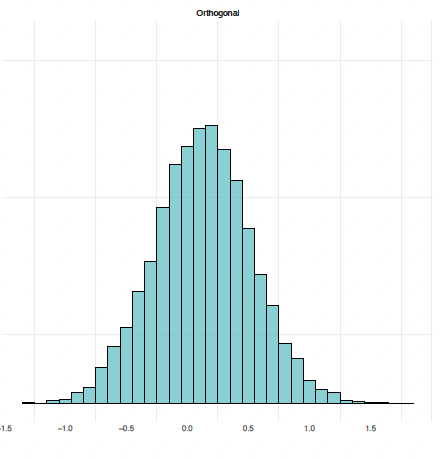
\includegraphics[width=0.3\textwidth]{Figures/orthogonal.png}
                    \end{center}
             \scriptsize       
            \textbf{Key Takeaways:}
            \begin{itemize}
                \item The naive LASSO-based estimator fails because it is not Neyman orthogonal, leading to slow bias convergence.
                \pause
                \item Double Lasso solves two separate prediction problems ($Y$ on $W$ and $D$ on $W$) and uses residuals to form an orthogonal moment condition.
                \pause
                \item Under approximate sparsity and proper tuning, Double Lasso achieves $\sqrt{n}$-rate inference and classical-style confidence intervals for the target parameter.
                \pause
                \item Neyman orthogonality is the key principle ensuring that errors in nuisance estimation do not propagate to first-order bias in the final estimate.
            \end{itemize}
        
            \end{frame}
   \section{Double Machine Learning in PLM}
   
   \begin{frame}{Partially Linear Model (PLM)}
    \textbf{Model Setup:}
    \begin{itemize}
        \item The PLM captures both linear and nonlinear relationships:
        \[
        Y = \beta D + g(X) + \epsilon, \quad \text{where } E[\epsilon | D, X] = 0.
        \]
        \pause
        \item Components:
        \begin{itemize}
            \item \(Y\): Outcome variable.
            \item \(D\): Regressor of interest (e.g., treatment or exposure).
            \item \(X\): High-dimensional control variables or features.
            \item \(g(X)\): Nonlinear component capturing the effect of \(X\).
        \end{itemize}
        \pause
        \item \(\beta\): Measures the predictive or causal effect of \(D\) on \(Y\), controlling for \(X\).
    \end{itemize}
    
    
    \end{frame}
    
    \begin{frame}{Residualized Vectors}
        \textbf{Partialling-out \(X\):}
        \begin{itemize}
            \item Define residualized \(Y\) and \(D\) by removing the influence of \(X\):
            \[
            \tilde{Y} := Y - \ell(X), \quad \tilde{D} := D - m(X),
            \]
            where:
            \[
            \ell(X) := E[Y | X], \quad m(X) := E[D | X].
            \]
            \pause
            \item Substituting into the PLM:
            \[
            \tilde{Y} = \beta \tilde{D} + \epsilon, \quad \text{with } E[\epsilon \tilde{D}] = 0.
            \]
        \end{itemize}
        
        \pause
        
        \textbf{Key Insight:}
        \begin{itemize}
            \item Residualization isolates the effect of \(D\) on \(Y\) by removing confounding through \(X\).
            \item The moment condition \(E[\tilde{Y} - \beta \tilde{D}]\tilde{D} = 0\) identifies \(\beta\).
        \end{itemize}
        \end{frame}
           
        \begin{frame}{FWL Partialling-Out for PLM}
            \textbf{Theorem}
            \begin{itemize}
                \item Suppose \(Y\), \(D\), and \(X\) have bounded second moments.
                \pause
                \item Then \(\beta\) is identified by the population regression of \(\tilde{Y}\) on \(\tilde{D}\):
                \[
                \beta := \arg \min_{b} E[(\tilde{Y} - b\tilde{D})^2].
                \]
                \pause
                \item Explicit solution:
                \[
                \beta = \frac{E[\tilde{Y} \tilde{D}]}{E[\tilde{D}^2]}.
                \]
            \end{itemize}
            
            \pause
            
            \textbf{Interpretation:}
            \begin{itemize}
                \item \(\beta\) is the regression coefficient of residualized \(Y\) on residualized \(D\), generalizing the Frisch-Waugh-Lovell theorem to PLMs.
                \item Residuals ensure confounding from \(X\) is removed.
            \end{itemize}
            \end{frame}
            \begin{frame}{Cross-Fitting and Overfitting}
                \begin{figure}
                    \centering
                    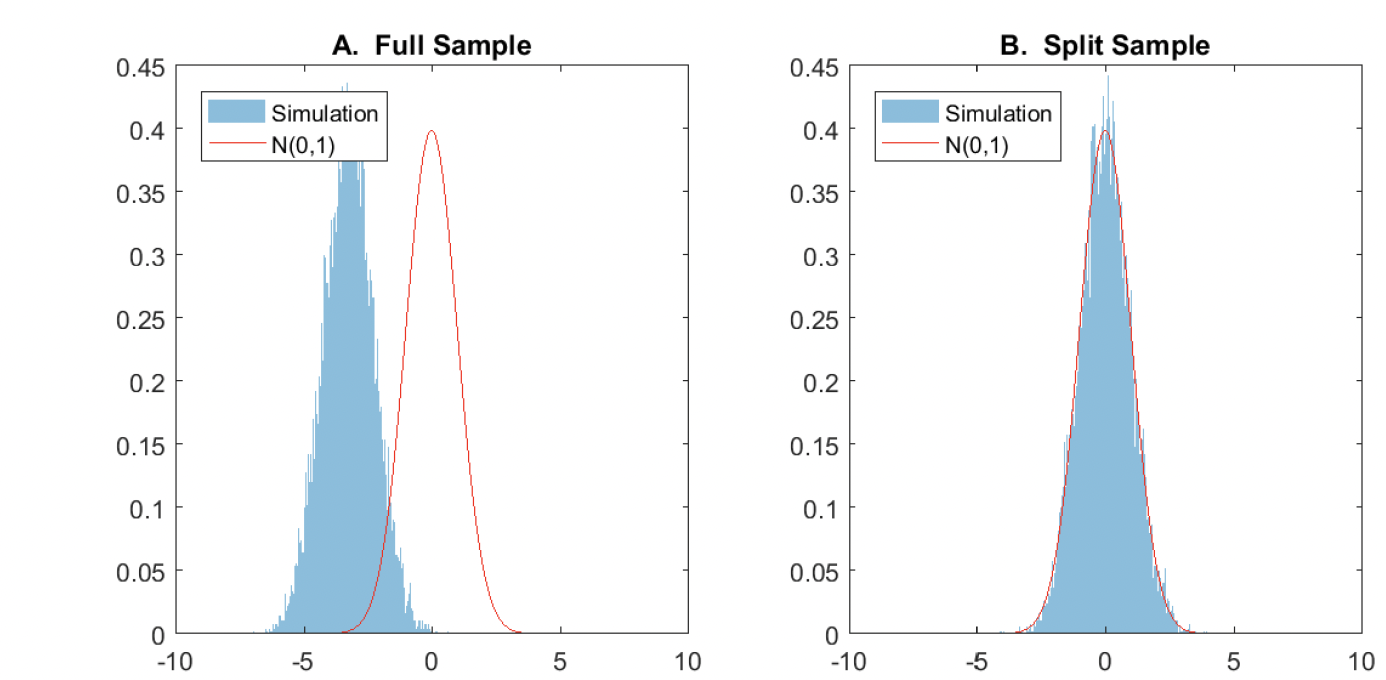
\includegraphics[width=0.5\textwidth]{Figures/overfitting.png}
                \end{figure}
                
                \pause
                \scriptsize
                \textbf{Why Cross-Fitting?}
                \begin{itemize}
                    \item Overfitting during the estimation of residualized quantities (e.g., \(\tilde{Y}, \tilde{D}\)) can introduce bias into the estimation of \(\beta\).
                    \pause
                    \item Data-driven tuning methods like cross-validation often lead to mild overfitting, as the same data is used repeatedly.
                    \pause
                    \item Cross-fitting mitigates this issue by using sample-splitting:
                    \begin{itemize}
                        \scriptsize
                        \item Nuisance parameters (\(\ell(X), m(X)\)) are estimated on one part of the data.
                        \item Residuals (\(\tilde{Y}, \tilde{D}\)) are computed on another.
                    \end{itemize}
                    \pause
                    \item Even when using simple learners like LASSO, cross-fitting is recommended unless theoretical penalty levels (\(\lambda\)) are used.
                \end{itemize}
                
                \pause
                
                \textbf{Practical Implication:}
                \begin{itemize}
                    \item Cross-fitting ensures robust inference by preventing overfitting from contaminating estimates of the parameter of interest.
                    \item Especially crucial when using complex machine learning methods.
                \end{itemize}
                \end{frame}
            \begin{frame}{Double Machine Learning (DML) Procedure}
                \textbf{Steps:}
                \begin{enumerate}
                    \item \textbf{Cross-Fitting:}
                    \begin{itemize}
                        \item Partition data into \(K\) folds: \(\{1, ..., n\} = \cup_{k=1}^K I_k\).
                        \item For each fold \(k\), estimate \(\ell(X)\) and \(m(X)\) using data outside \(I_k\).
                        \item Compute cross-fitted residuals for \(i \in I_k\):
                        \[
                        \tilde{Y}_i = Y_i - \ell^{[-k]}(X_i), \quad \tilde{D}_i = D_i - m^{[-k]}(X_i).
                        \]
                    \end{itemize}
                    \pause
                    \item \textbf{OLS Regression:}
                    \begin{itemize}
                        \scriptsize
                        \item Regress \(\tilde{Y}_i\) on \(\tilde{D}_i\) to estimate \(\beta\):
                        \[
                        \hat{\beta} = \frac{\frac{1}{n}\sum \tilde{Y}_i \tilde{D}_i}{\frac{1}{n}\sum \tilde{D}_i^2}.
                        \]
                    \end{itemize}
                    \pause
                    \scriptsize
                    \item \textbf{Inference:}
                    \begin{itemize}

                        \item Construct standard errors using:
                        \scriptsize
                        \[
                        \hat{V} = \left(\frac{1}{n}\sum \tilde{D}_i^2\right)^{-1}\left(\frac{1}{n}\sum \tilde{D}_i^2 \epsilon_i^2\right)\left(\frac{1}{n}\sum \tilde{D}_i^2\right)^{-1}.
                        \]
                        \item Confidence Interval:
                     \scriptsize
                        \[
                        \left[\hat{\beta} \pm 1.96 \cdot \sqrt{\frac{\hat{V}}{n}}\right].
                        \]
                    \end{itemize}
                \end{enumerate}
                \end{frame}



               
                                
                \begin{frame}{Summary and Extensions}
                    \textbf{Key Takeaways:}
                    \begin{itemize}
                        \item The PLM framework combines flexibility (nonlinearity via \(g(X)\)) with interpretability (linear effect of \(D\)).
                        \item DML ensures valid inference on \(\beta\) despite high-dimensional \(X\).
                        \item Cross-fitting mitigates overfitting from machine learning-based nuisance parameter estimation.
                    \end{itemize}
                    
                    \pause
                    
                    \textbf{When PLM Fails:}
                    \begin{itemize}
                        \item DML estimates the best linear predictor (BLP) of \(\tilde{Y}\) in terms of \(\tilde{D}\), even if PLM does not hold.
                        \item In this case, \(\beta\) captures an approximation of the effect of \(D\) on \(Y\).
                    \end{itemize}
                    \end{frame} 



           \section{Generic DML}         
                    \begin{frame}{Defining the Moment Condition}
                        \textbf{Key Ingredients}
                        \begin{itemize}
                            \item DML is based on the \textbf{method-of-moments} framework, targeting a low-dimensional parameter of interest, \(\theta_0\), defined via the moment condition:
                            \[
                            E[\psi(W; \theta_0, \eta_0)] = 0,
                            \]
                            where:
                            \begin{itemize}
                                \item \(\psi\): Score function.
                                \item \(W\): Data vector.
                                \item \(\theta_0\): Parameter of interest.
                                \item \(\eta_0\): Nuisance parameters (unknown high-dimensional functions).
                            \end{itemize}
                            \pause
                            \item \textbf{Interpretation:} \(\theta_0\) is identified when the above equation holds.
                        \end{itemize}
                        \end{frame}
                        
                        \begin{frame}{Neyman Orthogonality}
                        \textbf{Key Concept}
                        \begin{itemize}
                            \item A score function \(\psi(W; \theta, \eta)\) satisfies \textbf{Neyman orthogonality} if:
                            \[
                            \frac{\partial}{\partial \eta} E[\psi(W; \theta_0, \eta)]\bigg|_{\eta=\eta_0} = 0.
                            \]
                            \pause
                            \item \textbf{Importance:} Eliminates first-order bias from errors in the nuisance parameter estimates, \(\hat{\eta}\).
                        \end{itemize}
                       
                        \end{frame}
                        
                        \begin{frame}{Gateaux Derivative}
                        \textbf{Definition}
                        \begin{itemize}
                            \item The \textbf{Gateaux derivative} formalizes sensitivity to small perturbations:
                            \[
                            \frac{\partial}{\partial \eta} E[\psi(W; \theta, \eta)][\Delta] := \frac{\partial}{\partial t} E[\psi(W; \theta, \eta + t\Delta)]\bigg|_{t=0}.
                            \]
                            \pause
                            \item \textbf{Implication:} Neyman orthogonality implies:
                            \[
                            \frac{\partial}{\partial \eta} E[\psi(W; \theta_0, \eta_0)][\Delta] = 0, \quad \forall \Delta.
                            \]
                            \pause
                            \item \textbf{Admissible Directions:} \(\Delta\) is admissible if \(\eta_0 + t\Delta\) stays in the parameter space for small \(t\).
                        \end{itemize}
                        \end{frame}
                        
                        \begin{frame}{Good Learners for Nuisance Functions}
                        \textbf{Requirements for High-Quality Learners}
                        \begin{itemize}
                            \item Learners must approximate the true nuisance parameters \(\eta_0\) well:
                            \[
                            n^{1/4} \|\hat{\eta} - \eta_0\|_{L^2} \approx 0.
                            \]
                            \pause
                            \item Examples of Machine Learning Methods:
                            \begin{enumerate}
                                \item \textbf{LASSO:} For sparsely parameterized \(\eta_0\).
                                \item \textbf{Random Forests:} For tree-like structures in \(\eta_0\).
                                \item \textbf{Deep Neural Networks:} For \(\eta_0\) approximable by sparse deep nets.
                                \item \textbf{Ensemble Models:} Combining methods to leverage strengths of each.
                            \end{enumerate}
                            \pause
                            \item Cross-validation and careful tuning are critical for robust performance.
                        \end{itemize}
                        \end{frame}
                        
                        \begin{frame}{Cross-Fitting}
                        \textbf{Why Cross-Fitting?}
                        \begin{itemize}
                            \item Prevents \textbf{overfitting}, which occurs when nuisance parameter estimates are correlated with the same data used for inference.
                            \pause
                            \item Mechanism:
                            \begin{enumerate}
                                \item Split data into \(K\) folds.
                                \item Use \(K-1\) folds to estimate nuisance parameters (\(\hat{\eta}\)).
                                \item Use the left-out fold to compute residuals and estimate the target parameter.
                            \end{enumerate}
                            \pause
                            \item \textbf{Outcome:} Avoids biases arising from overfitting complex machine learning methods.
                        \end{itemize}
                        \end{frame}
                        
                        \begin{frame}{Example 1: Partially Linear Model (PLM)}
                        \textbf{Moment Condition for PLM}
                        \[
                        \psi(W; \theta, \eta) = \left(Y - \ell(X) - \theta(D - m(X))\right)(D - m(X)).
                        \]
                        \begin{itemize}
                            \item \(W = (Y, D, X)\): Observable variables.
                            \item \(\eta = (\ell, m)\): Nuisance parameters.
                            \begin{itemize}
                                \item \(\ell(X) = E[Y | X]\), \(m(X) = E[D | X]\).
                            \end{itemize}
                        \end{itemize}
                        \pause
                        \textbf{Neyman Orthogonality}
                        \begin{itemize}
                            \item Using elementary calculations:
                            \[
                            \frac{\partial}{\partial \eta} E[\psi(W; \theta, \eta)]\big|_{\eta=\eta_0} = 0.
                            \]
                        \end{itemize}
                        \pause
                        \textbf{Interpretation:} \(\psi(W; \theta, \eta)\) generalizes residualization in linear models, enabling robust inference.
                        \end{frame}
                        
                        \begin{frame}{Example 2: Doubly Robust IPW}
                        \textbf{Doubly Robust IPW Estimator}
                        \[
                        \psi(W; \theta, \eta) = \left(g(1, X) - g(0, X)\right) + H(D, X)(Y - g(D, X)) - \theta,
                        \]
                        where:
                        \[
                        H(D, X) = \frac{D}{m(X)} - \frac{(1-D)}{1-m(X)}.
                        \]
                        \pause
                        \begin{itemize}
                            \item \(g(D, X) = E[Y | D, X]\), \(m(X) = P[D=1 | X]\).
                            \item nuisance parameters: \(\eta = (g, m)\).
                            \item Neyman Orthogonality:
                            \[
                            \frac{\partial}{\partial \eta} E[\psi(W; \theta, \eta)] = 0.
                            \]
                        \end{itemize}
                        \end{frame}
                        
                        \begin{frame}{Generic DML Algorithm}
                        
                        \begin{enumerate}
                            \item \textbf{Input:} Data \(\{W_i\}_{i=1}^n\), Neyman orthogonal score \(\psi(W; \theta, \eta)\), and machine learning methods for \(\eta\).
                            \pause
                            \item \textbf{Cross-Fitting:}
                            \begin{itemize}
                                \item Split data into \(K\) folds.
                                \item Train \(\hat{\eta}[k]\) on \(K-1\) folds and compute expectations on the left-out fold.
                            \end{itemize}\pause
                            \item \textbf{Moment Estimation:}
                            \[
                            \hat{M}(\theta, \hat{\eta}) = \frac{1}{n} \sum_{i=1}^n \psi(W_i; \theta, \hat{\eta}[k(i)]).
                            \]
                            
                            \item \textbf{Variance and Confidence Intervals:}
                            
                            \begin{itemize}\scriptsize
                                
                                    \item Estimate the asymptotic variance of \(\hat{\theta}\) as:
                                    \[
                                        \hat{V} = \frac{1}{n} \sum_{i=1}^n [\hat{\phi}(W_i) \hat{\phi}(W_i)'] 
                                        - \frac{1}{n} \sum_{i=1}^n [\hat{\phi}(W_i)] \frac{1}{n} \sum_{i=1}^n [\hat{\phi}(W_i)]', \quad
                                        \hat{\phi}(W_i) = -\hat{J}_0^{-1} \psi(W_i; \hat{\theta}, \hat{\eta}[k(i)]), \,
                                        \hat{J}_0 = \frac{\partial}{\partial \theta} \frac{1}{n} \sum_{i=1}^n \psi(W_i; \hat{\theta}, \hat{\eta}[k(i)]).
                                        \]
                                    
                                        \pause
                                \item Confidence interval:
                                \[
                                [\hat{\theta} \pm z_{1-\alpha/2} \sqrt{\hat{V}/n}].
                                \]
                            \end{itemize}
                        \end{enumerate}
                        \end{frame}

\end{document}


































 


